\documentclass[tikz]{standalone}

\usetikzlibrary{calc}

\begin{document}


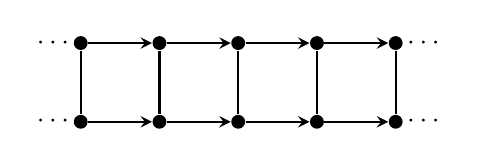
\begin{tikzpicture}[>=stealth]

\foreach \x in {0,...,4} {
	\foreach \y in {0,1} {
		\node [fill=black,black,circle,inner sep=0pt,minimum size=.5em] (n\x-\y) at (\x,\y) {};
	}
}

\foreach \x in {0,...,3} {
	
	\pgfmathtruncatemacro{\j}{\x + 1};
	
	\node [fill=none,circle,inner sep=0pt,minimum size=.5em]
	(b\x) at ($(n\x-0)!0.5!(n\j-1)$) {};
	
	\draw [->,thick] (n\x-1) to (n\j-1);
	\draw [->,thick] (n\x-0) to (n\j-0);
}

\foreach \x in {0,...,4} {
	\draw [thick] (n\x-0) to (n\x-1);
}

\node () [left of= n0-0,node distance=1em] {$\cdots$};
\node () [left of= n0-1,node distance=1em] {$\cdots$};
\node () [right of= n4-0,node distance=1em] {$\cdots$};
\node () [right of= n4-1,node distance=1em] {$\cdots$};

\end{tikzpicture}


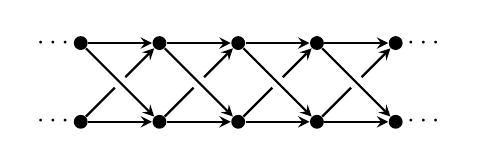
\begin{tikzpicture}[>=stealth]

\foreach \x in {0,...,4} {
	\foreach \y in {0,1} {
		\node [fill=black,black,circle,inner sep=0pt,minimum size=.5em] (n\x-\y) at (\x,\y) {};
	}
}

\foreach \x in {0,...,3} {
	
	\pgfmathtruncatemacro{\j}{\x + 1};
	
	\node [fill=none,circle,inner sep=0pt,minimum size=.5em]
		(b\x) at ($(n\x-0)!0.5!(n\j-1)$) {};

	\draw [->,thick] (n\x-1) to (n\j-1);
	\draw [->,thick] (n\x-0) to (n\j-0);
	
	\draw [->,thick] (n\x-1) -- (n\j-0);
	\draw [->,thick] (n\x-0) -- (b\x) -- (n\j-1);

}

\node () [left of= n0-0,node distance=1em] {$\cdots$};
\node () [left of= n0-1,node distance=1em] {$\cdots$};
\node () [right of= n4-0,node distance=1em] {$\cdots$};
\node () [right of= n4-1,node distance=1em] {$\cdots$};

\end{tikzpicture}
\end{document}

